\documentclass[a4paper]{article}

%% Language and font encodings
\usepackage[english]{babel}
\usepackage[utf8x]{inputenc}
\usepackage[T1]{fontenc}

%% Sets page size and margins
\usepackage[a4paper,top=3cm,bottom=2cm,left=3cm,right=3cm,marginparwidth=1.75cm]{geometry}

%% Useful packages
\usepackage{amsmath}
\usepackage{graphicx}
\usepackage[colorinlistoftodos]{todonotes}
\usepackage[colorlinks=true, allcolors=blue]{hyperref}

\title{Actividad VI}
\author{Jose Pablo Montaño}
\date{12 de Abril 2018}

\begin{document}
\maketitle


\section{Introduccion}

En esta ocacion se realizo un trabajo en el cual se modelo el comportamiento de dos resortes con masas colgados de forma veritical uno atado del otro. Para esto se utilizaron las ecuaciones diferenciales que se presentaron en el documento de Fay y Graham.

\subsection{Seccion 1 de Fay y Graham}


Los requerimentos para iniciar con las ecuaciones diferenciales esta cambiando de saber resolver una variedad de ecuaciones con diferentes tecnicas a enfatizar el uso de sistemas que resulevan estas ecuaciones. Para ser espesificos existe un gran enfoque en la resolucion de sistemas no lineales con algoritmos numericos.
\linebreak

En este articulo se trata de modelar y reolver una cituacion referente a la ley de Hooke con resortes con dos grados de libertad modelados con ecuaciones no lineales. Los resortes se encuentran acoplados uno a otro con un peso atado a cada uno respectivamente. El movimineot de esas masas se puede modelar con una ecuacion de cuarto orden. En este trabajo se puede apreciar que moviminetos interesantes surgen de la no linealidad. 


\subsection{Seccion 1 de Fay y Graham}

El sistema a modelar consiste en un resorte con una masa que a su vez esta unido a otro resorte con una masa, ambos colocados de forma vertical, como se muestra en la imagen.

\begin{figure}[ht!]
\centering
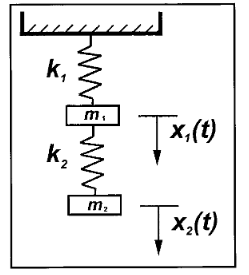
\includegraphics[width=0.3\textwidth]{Resorte.png}
\end{figure}

Asumimos que k1 y k2 son las constantes del reosrte y que l1 y l2 son las enlongaciones de este, lo cual cumple con la ley de hooke. Haciendo la consideracion de que el primer sistema de resorte masa no solo siente su peso sino tambien el del resorte dos y que el resorte dos solo siente su propio peso, podemos llegar a la siguiente ecuacion.

\begin{figure}[ht!]
\centering
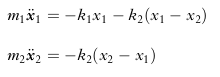
\includegraphics[width=0.3\textwidth]{E1.png}
\end{figure}

Esto lo podemos colocar en jupyter lab de la siguiente forma. 

\begin{verbatim}

def vectorfield(w, t, p):
    """
    Defines the differential equations for the coupled spring-mass system.

    Arguments:
        w :  vector of the state variables:
                  w = [x1,y1,x2,y2]
        t :  time
        p :  vector of the parameters:
                  p = [m1,m2,k1,k2,L1,L2,b1,b2]
    """
    x1, y1, x2, y2 = w
    m1, m2, k1, k2, L1, L2, b1, b2 = p

    # Create f = (x1',y1',x2',y2'):
    f = [y1,
         (-b1 * y1 - k1 * (x1) + k2 * (x2 - x1)) / m1,
         y2,
         (-b2 * y2 - k2 * (x2 - x1)) / m2]
    return f


\end{verbatim}

Utilizamos odient para resolver la ecuacion diferencial de la siguiente forma

\begin{verbatim}
from scipy.integrate import odeint
import numpy as np
import math

\end{verbatim}

Despues utilizamos las espesificaciones dadas para cada ejemplo.

Example 2.1.Describe the motion for spring constants K1=6 and K2=4 with initial conditions (x1(0),y1(0),x2(0),y2(0))=(1,0,2,0)  

\begin{figure}[ht!]
\centering
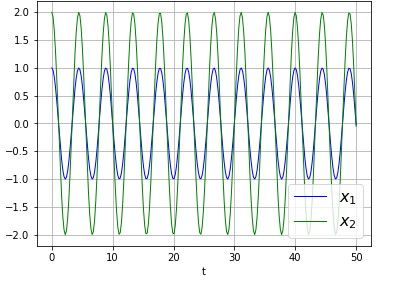
\includegraphics[width=0.3\textwidth]{2_1_1.png}
\end{figure}

\begin{figure}[ht!]
\centering
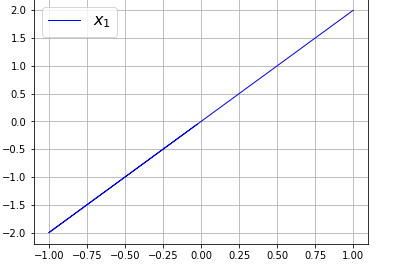
\includegraphics[width=0.3\textwidth]{2_1_2.png}
\end{figure}

\begin{figure}[ht!]
\centering
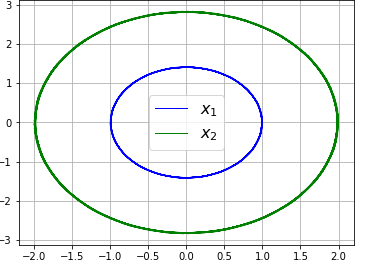
\includegraphics[width=0.3\textwidth]{2_1_3.png}
\end{figure}

\newpage


Soluciones particulares usadas para calcular el error 

\begin{verbatim}
X1(t)=cos((2t)**1/2))

X2(t)=2cos((2t)**1/2))
\end{verbatim}


\begin{figure}[ht!]
\centering
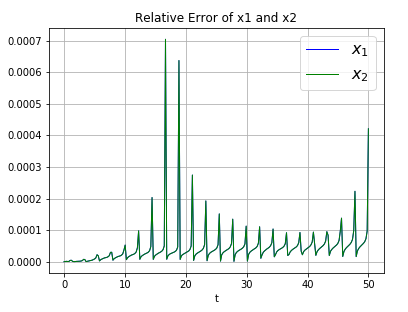
\includegraphics[width=0.3\textwidth]{2_1_4.png}
\end{figure}

%\newpage

Example 2.2.Describe the motion for spring constants K1=6 and K2=4 with initial conditions (x1(0),y1(0),x2(0),y2(0))=(-2,0,1,0)  

\begin{figure}[ht!]
\centering
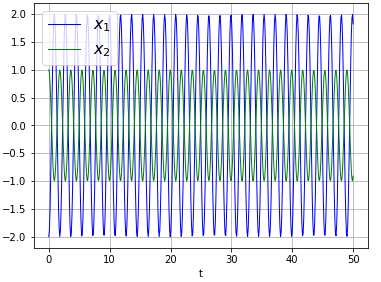
\includegraphics[width=0.3\textwidth]{2_2_1.png}
\end{figure}

\begin{figure}[ht!]
\centering
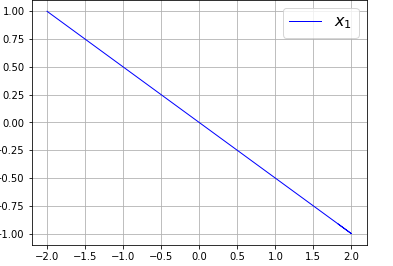
\includegraphics[width=0.3\textwidth]{2_2_2.png}
\end{figure}

\newpage

Soluciones particulares usadas para calcular el error 

\begin{verbatim}
X(t)=-2cos2((3t)**1/2))

X2(t)=cos2((3t)**1/2))
\end{verbatim}


\begin{figure}[ht!]
\centering
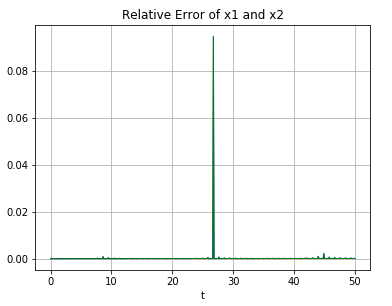
\includegraphics[width=0.3\textwidth]{2_2_3.png}
\end{figure}


Example 2.3.Describe the motion for spring constants K1=.4 and K2=1.808 with initial conditions (x1(0),y1(0),x2(0),y2(0))=(1/2,0,-1/2,7/10)  

\begin{figure}[ht!]
\centering
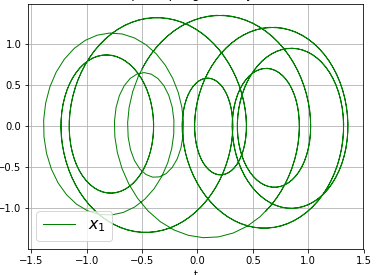
\includegraphics[width=0.3\textwidth]{2_3_1.png}
\end{figure}

\begin{figure}[ht!]
\centering
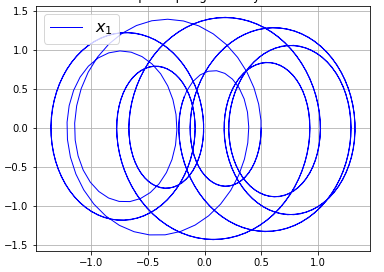
\includegraphics[width=0.3\textwidth]{2_3_2.png}
\end{figure}

\begin{figure}[ht!]
\centering
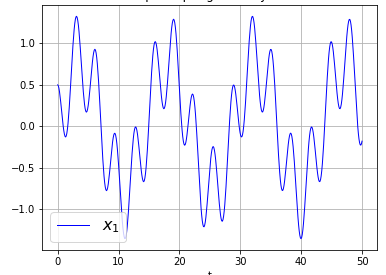
\includegraphics[width=0.3\textwidth]{2_3_3.png}
\end{figure}

\begin{figure}[ht!]
\centering
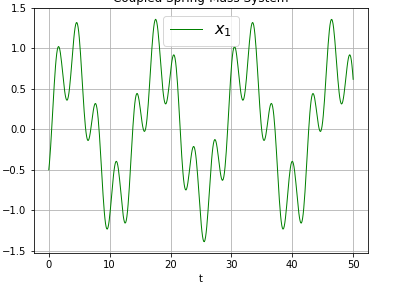
\includegraphics[width=0.3\textwidth]{2_3_4.png}
\end{figure}

\begin{figure}[ht!]
\centering
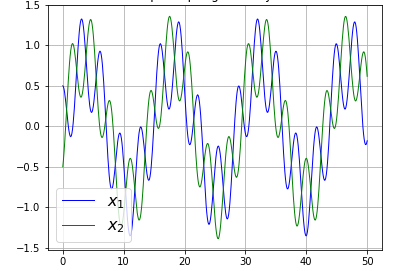
\includegraphics[width=0.3\textwidth]{2_3_5.png}
\end{figure}

\begin{figure}[ht!]
\centering
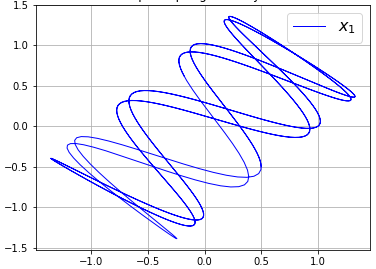
\includegraphics[width=0.3\textwidth]{2_3_6.png}
\end{figure}

\newpage

En este modelo tambien se puede incorporar un cierto amortiguamiento en el movimiento de los resortes lo cual se modela haciendo una pequeña modificacion a la ecuacion diferencial que modela el movimiento de estos como se muestra a continuacion.

\begin{figure}[ht!]
\centering
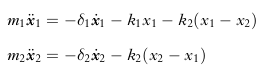
\includegraphics[width=0.3\textwidth]{E2.png}
\end{figure}

El codigo donde se definio el vector de ecuaciones que describe este movimiento se planteo como sigue.

\begin{verbatim}



def vectorfield(w, t, p):
    """
    Defines the differential equations for the coupled spring-mass system.

    Arguments:
        w :  vector of the state variables:
                  w = [x1,y1,x2,y2]
        t :  time
        p :  vector of the parameters:
                  p = [m1,m2,k1,k2,L1,L2,b1,b2]
    """
    x1, y1, x2, y2 = w
    m1, m2, k1, k2, L1, L2, b1, b2 = p

    # Create f = (x1',y1',x2',y2'):
    f = [y1,
         (-b1 * y1 - k1 * (x1) - k2 * (x1 - x2)),
         y2,
         (-b2 * y2 - k2 * (x2 - x1))]
    return f

\end{verbatim}

Example 2.4.Describe the motion for spring constants K1=.4 and K2=1.808 with initial conditions (x1(0),y1(0),x2(0),y2(0))=(1/2,0,-1/2,7/10)  

\begin{figure}[ht!]
\centering
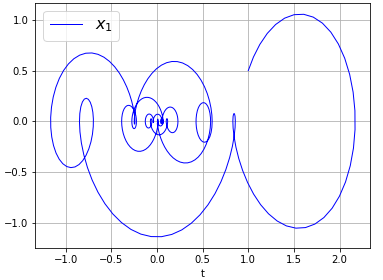
\includegraphics[width=0.3\textwidth]{2_4_1.png}
\end{figure}

\begin{figure}[ht!]
\centering
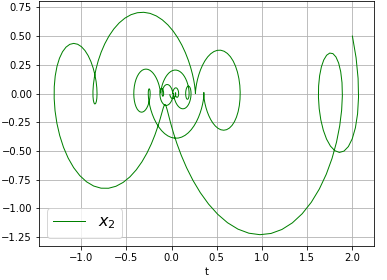
\includegraphics[width=0.3\textwidth]{2_4_2.png}
\end{figure}

\begin{figure}[ht!]
\centering
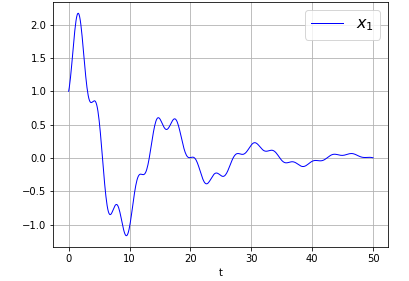
\includegraphics[width=0.3\textwidth]{2_4_3.png}
\end{figure}

\begin{figure}[ht!]
\centering
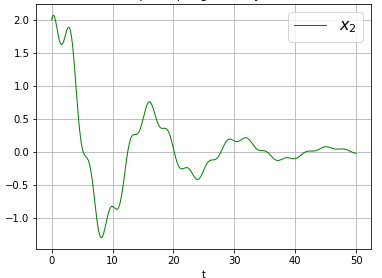
\includegraphics[width=0.3\textwidth]{2_4_4.png}
\end{figure}

\begin{figure}[ht!]
\centering
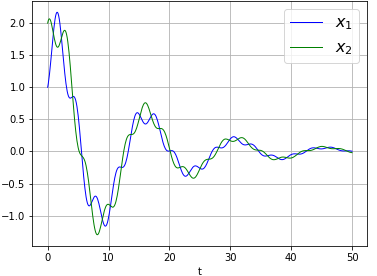
\includegraphics[width=0.3\textwidth]{2_4_5.png}
\end{figure}

\begin{figure}[ht!]
\centering
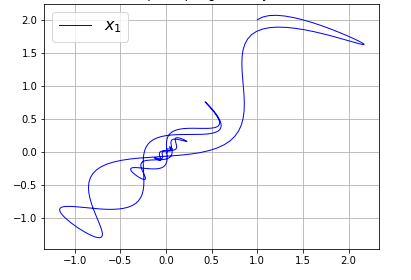
\includegraphics[width=0.3\textwidth]{2_4_6.png}
\end{figure}

    ¿En general te pareció interesante esta actividad de modelación matemática? ¿Qué te gustó mas? ¿Qué no te gustó?
    \linebreak
    
    Fue interesante como se puede procesar la informacion rapidamente con el uso de herramientas computacionales y como estas ya estan listas y realmente no requieren mucha programacion. Me gusto que hubiese un ejemplo muy pareciso inicial y no me gusto que no hubiera un ejemplo para obtener el error.
    \linebreak
    
    La cantidad de material te pareció ¿bien?, ¿suficiente?, ¿demasiado
    \linebreak
    Aunque considero que hubo ahora un poco más de material de apoyo sigo pensando que es necesario un par de clases de introduccion.
    \linebreak
    
    ¿Cuál es tu primera impresión de Jupyter Lab? 
    \linebreak
    Es como Jupyter notebook pero con otra interface
    \linebreak
    
    Respecto al uso de funciones de SciPy, ¿ya habías visto integración numérica en tus cursos anteriores? ¿Cuál es tu experiencia
    \linebreak
    Ya habia visto integracion numerica en otros cursos, sin embargo fue más facil con SciPy.
    \linebreak
   
    
    El tema de sistema de masas acopladas con resortes, ¿ya lo habías resuelto en tu curso de Mecánica 2? 
    \linebreak
    No que yo recuerde.
    \linebreak|
    ¿Qué le quitarías o agregarías a esta actividad para hacerla más interesante y divertida? 
    
    Le agregaria una clase de introduccion.


\end{document}

